\documentclass{beamer}
\usepackage[finnish]{babel}
\usepackage[T1]{fontenc}
\usepackage[utf8]{inputenc}
\usepackage{tikz}
\usetheme{Warsaw}
\title[Data assimilation in an elastic friction model]{Data assimilation in an elastic friction model}
\author{Tom Gustafsson}
\date{20. September 2012}
\begin{document}

\begin{frame}
\titlepage
\end{frame}

\begin{frame}{Question}

\begin{itemize}
\item Is it possible to estimate weakly known parameters from a simple elastic friction model by using the tools of data assimilation?
\end{itemize}

\begin{figure}
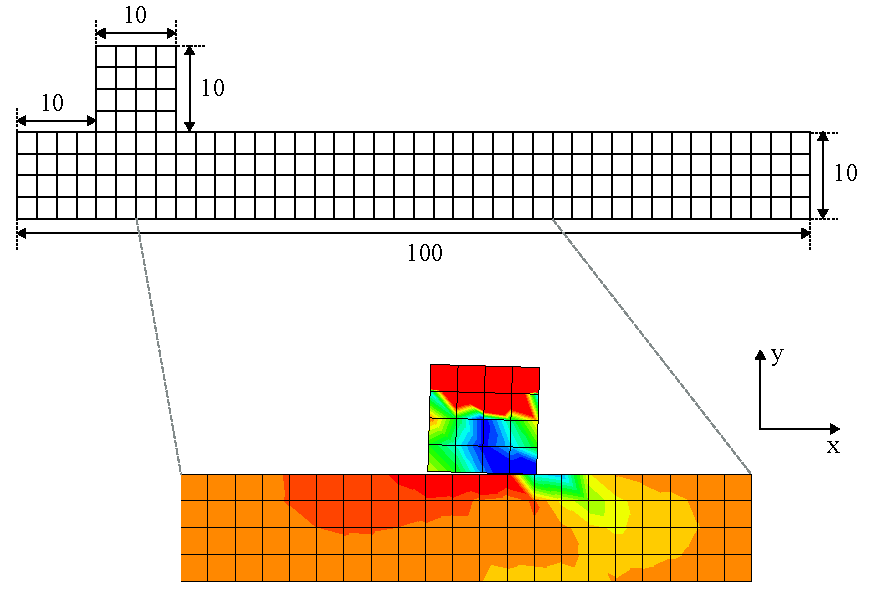
\includegraphics[width=8cm]{fretting_mesh.pdf}
\end{figure}

\end{frame}

\begin{frame}{Model, 2D}

\begin{itemize}
\item Initial setting: Block, slab
\item Boundary conditions
\end{itemize}

\begin{figure}
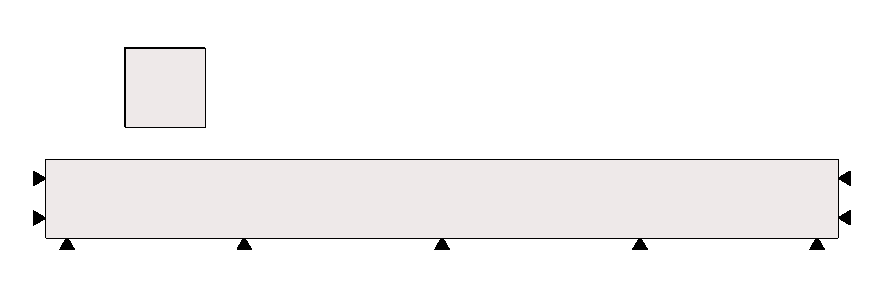
\includegraphics[width=10cm]{fretting_geom.pdf}
\end{figure}

\begin{itemize}
\item Abaqus/Standard 6.12-1, simulations on CSC
\end{itemize}

\end{frame}

\begin{frame}{Steps of the simulation}

\begin{itemize}
\item Step 1: 5 kN force acting downwards
\end{itemize}

\begin{figure}
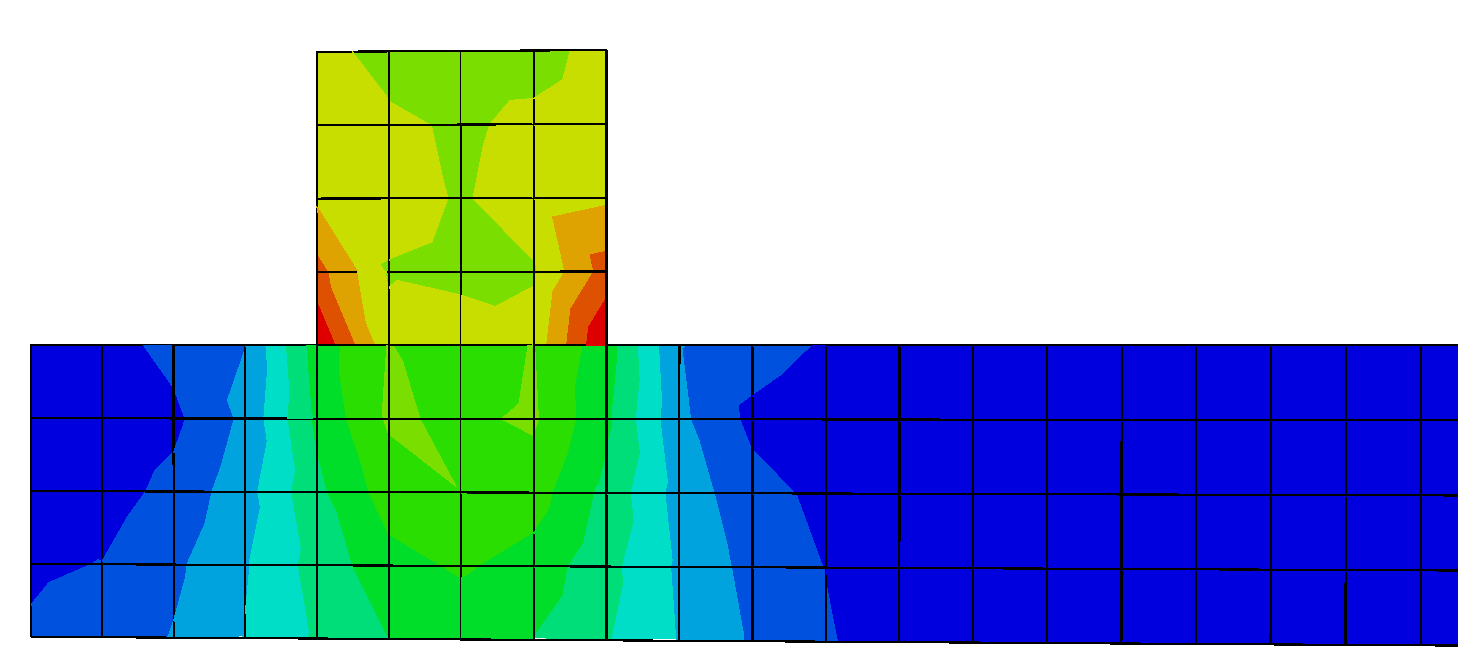
\includegraphics[width=9cm]{mises.pdf}
\end{figure}

\begin{itemize}
\item Step 2: Displacement of block's upper boundary by 70 cm to the right
\end{itemize}

\end{frame}

\begin{frame}{Steps of the simulation: displacement of the block}

\begin{itemize}
\item Done by using boundary conditions. Thus, a "slow displacement"
\end{itemize}

\begin{figure}
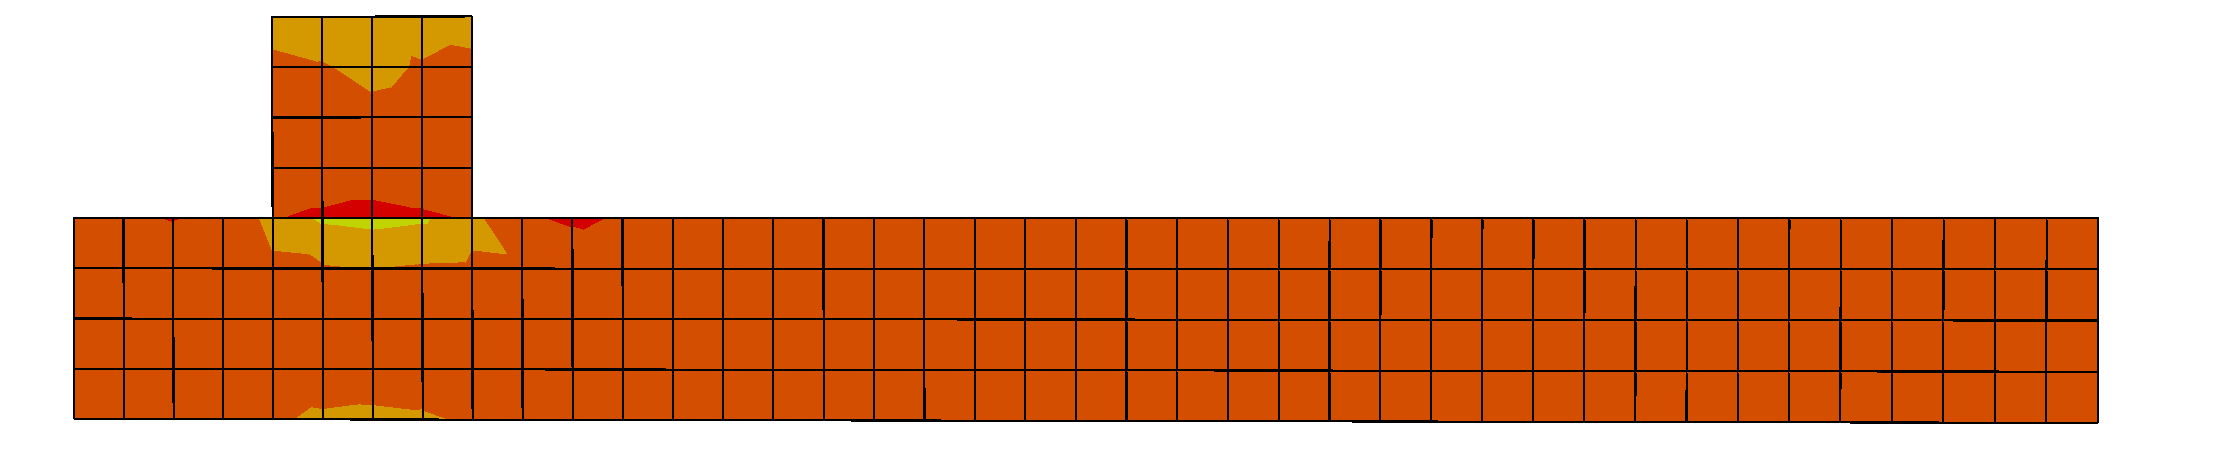
\includegraphics[width=10cm]{anim1.pdf}\\
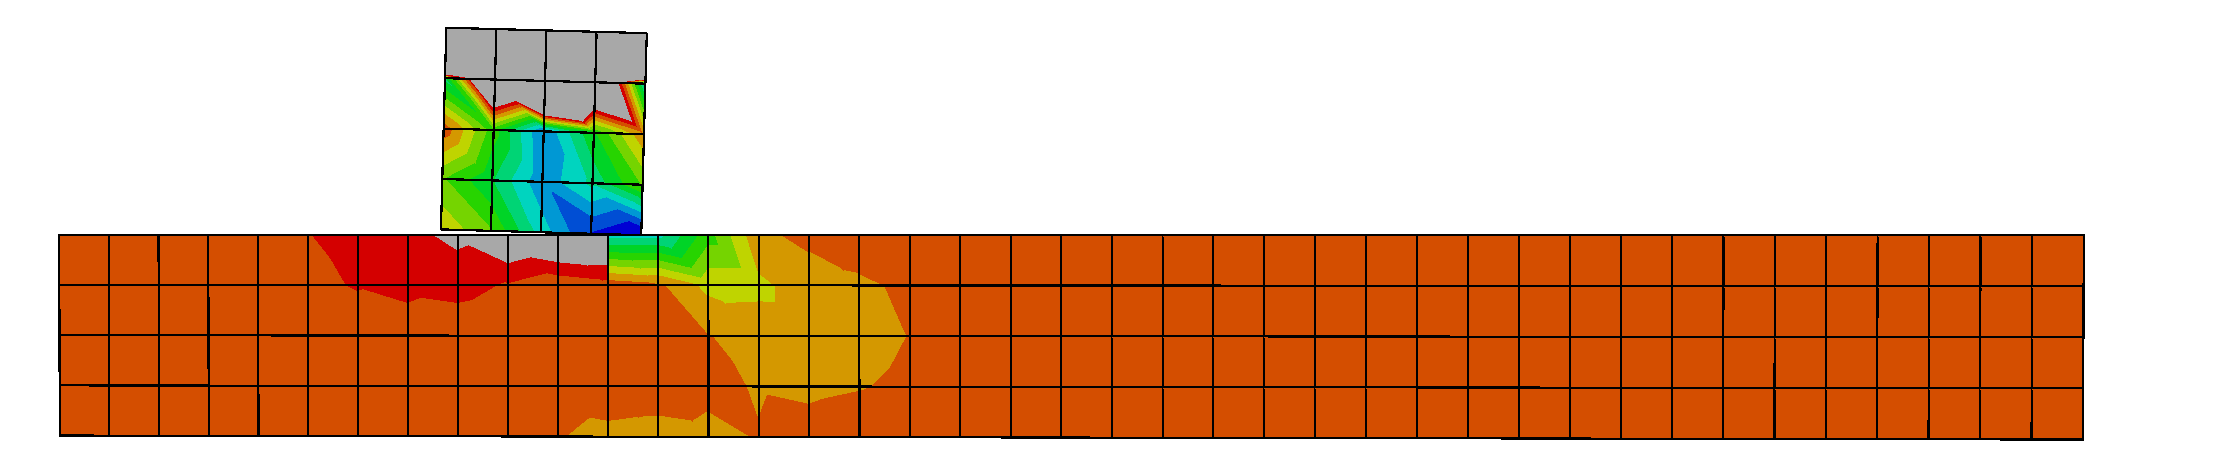
\includegraphics[width=10cm]{anim2.pdf}
\end{figure}

\end{frame}

\begin{frame}{Steps of the simulation: displacement of the block, 2}

\begin{figure}
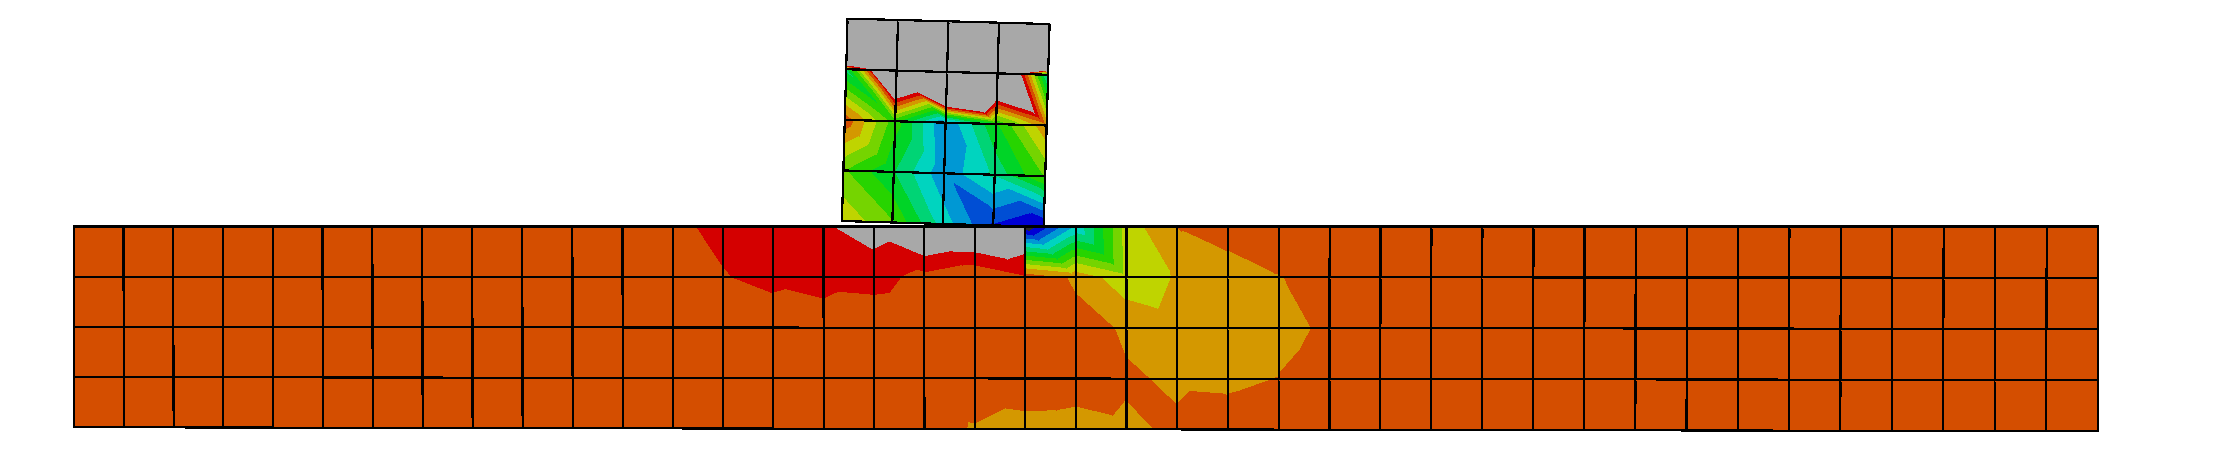
\includegraphics[width=10cm]{anim3.pdf}\\
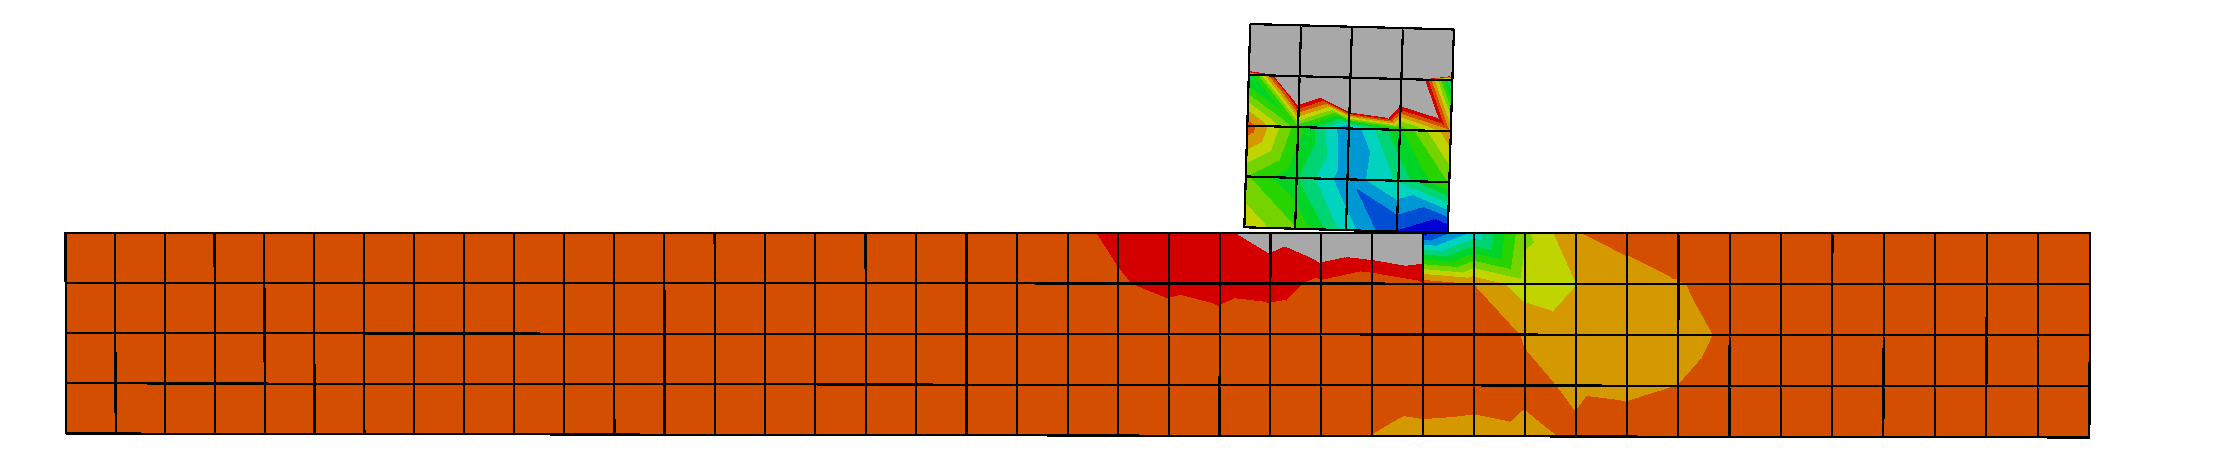
\includegraphics[width=10cm]{anim4.pdf}\\
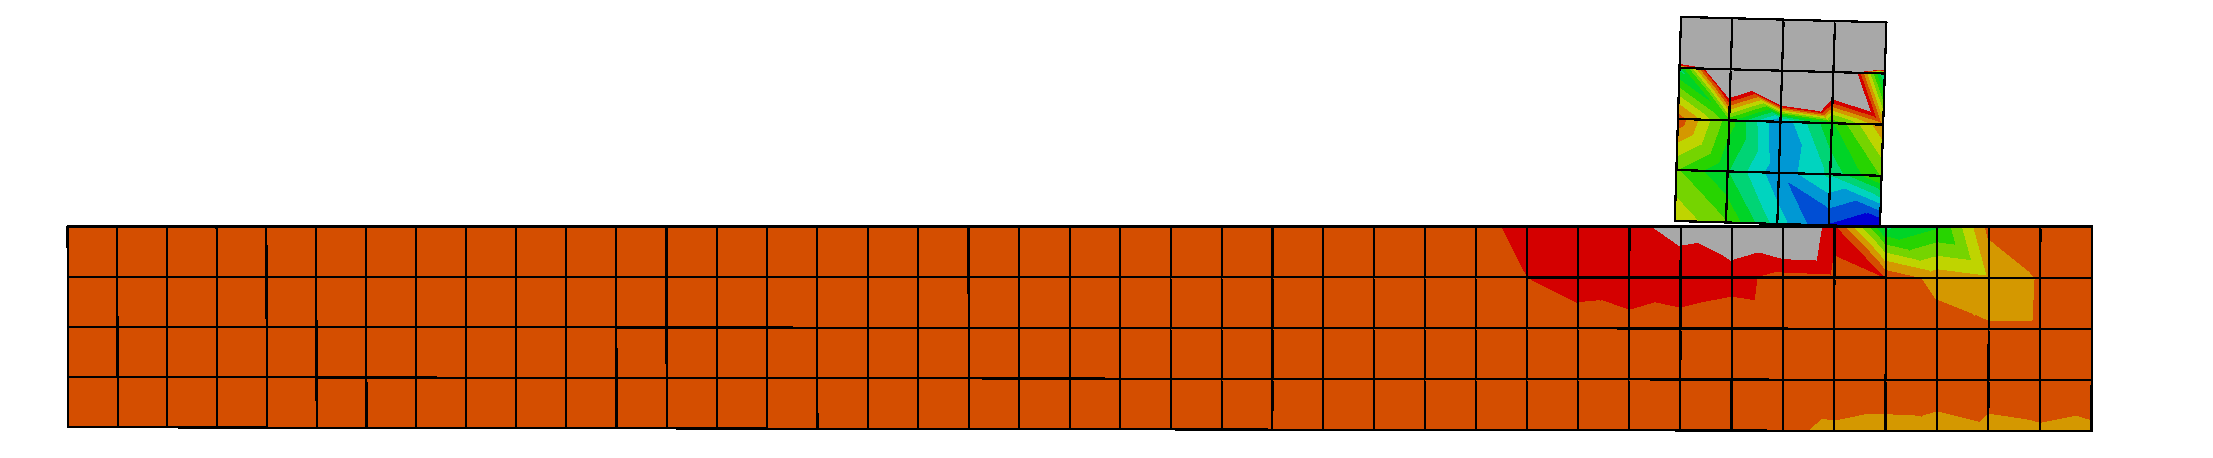
\includegraphics[width=10cm]{anim5.pdf}
\end{figure}

\end{frame}

\begin{frame}{Inversion problem}

\begin{itemize}
\item Attempting to estimate friction coefficient $\mu$
\item As \emph{a priori} data: $x$ directional stress in chosen measurement points\\($\sim$ strain gauge)
\end{itemize}

\begin{figure}
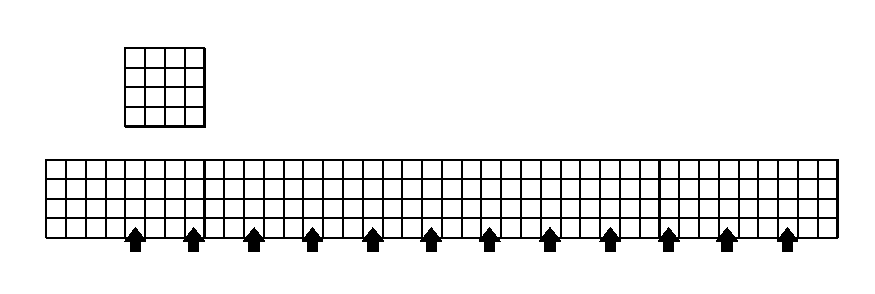
\includegraphics[width=10cm]{fretting_geom_meas.pdf}
\end{figure}

%\begin{itemize}
%\item Mittadata synteettistä
%\end{itemize}

\end{frame}

%\begin{frame}{Synteettisen mittadatan generointi}

%\begin{itemize}
%\item Minimoidaan inversiorikosta $\rightarrow$ mittadata tiheämmästä verkosta
%\end{itemize}

%\begin{figure}
%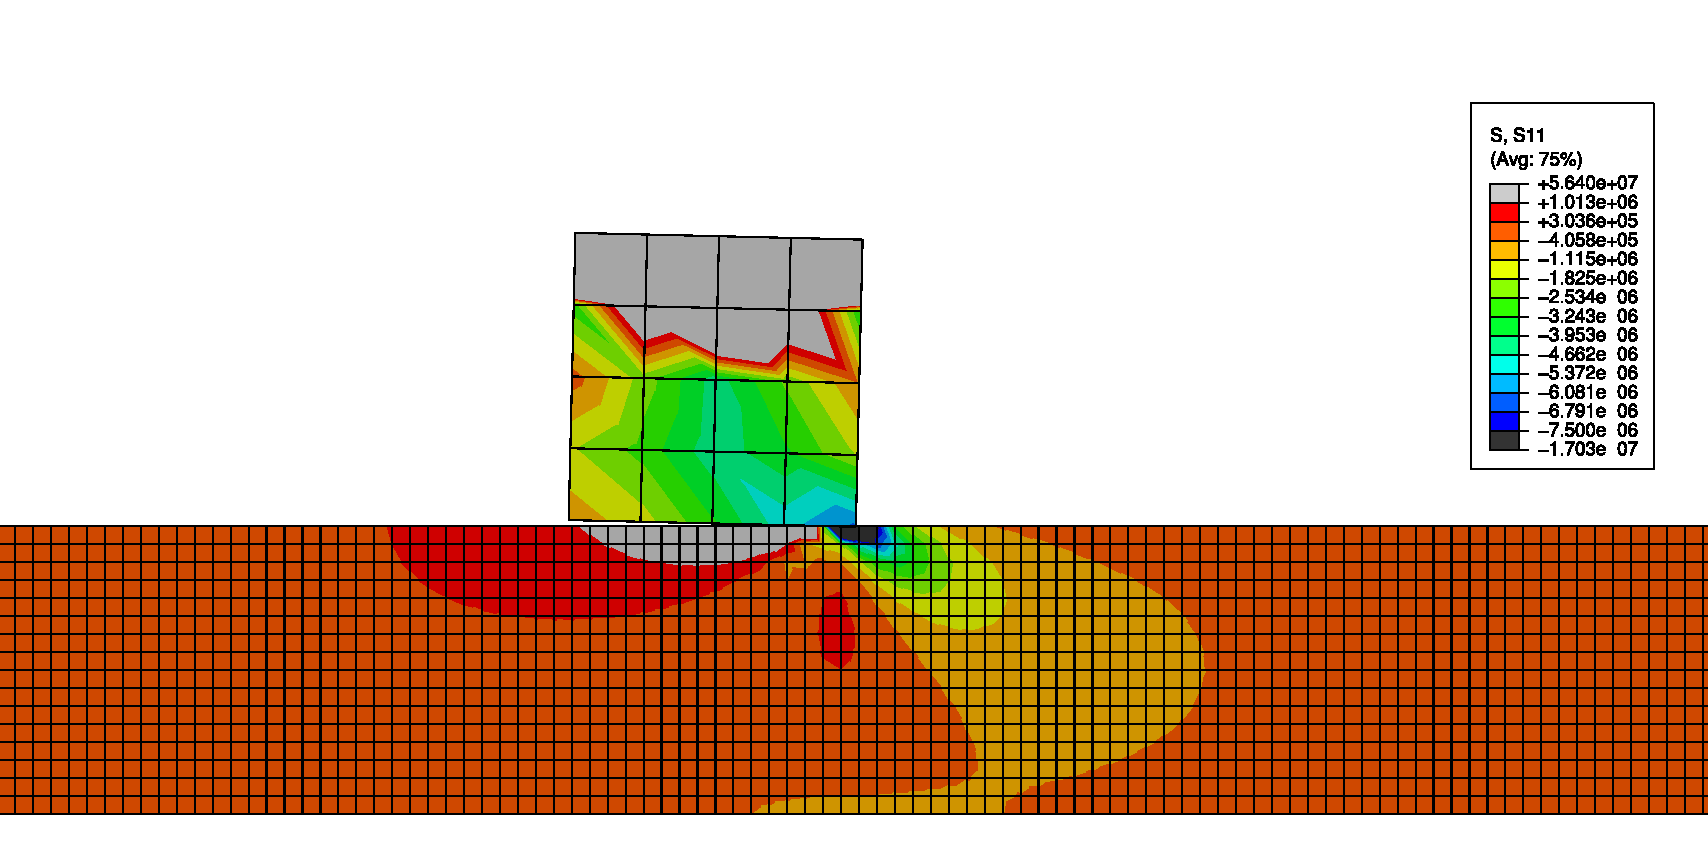
\includegraphics[width=10cm]{finer_mesh.pdf}
%\end{figure}

%\begin{itemize}
%\item Miten verrata tiheämmän ja harvemman verkon antamia jännityksiä?
%\end{itemize}

%\end{frame}

%\begin{frame}{Synteettisen mittadatan generointi 2}

%\begin{figure}
%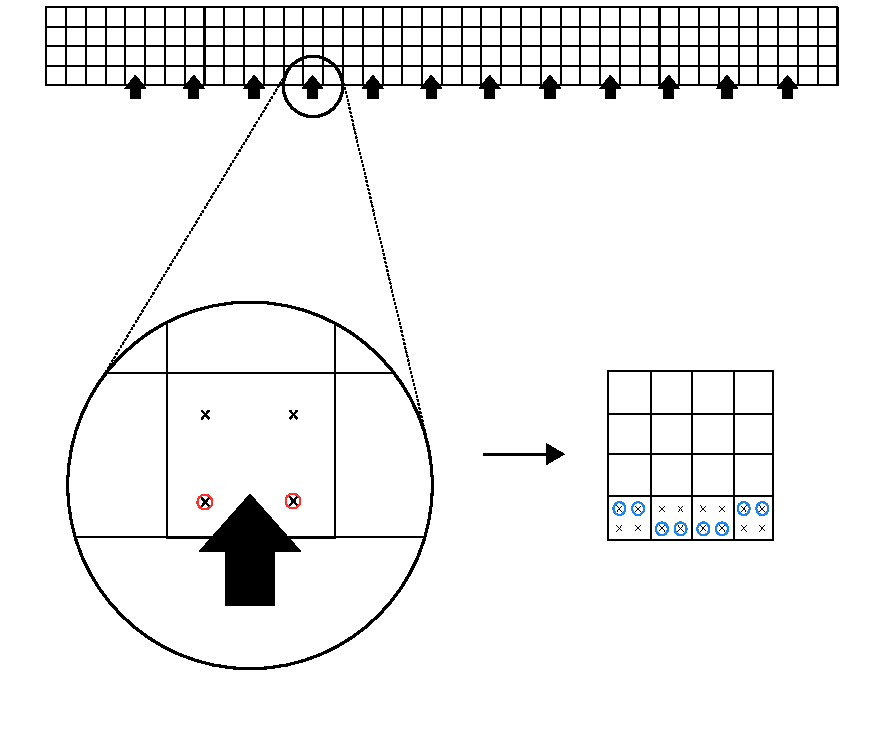
\includegraphics[width=10cm]{fretting_meas_tarkempi.pdf}
%\end{figure}

%\end{frame}

%\begin{frame}{Ongelman yhteenveto}

%\begin{itemize}
%\item Estimoitava suure: Kitkakerroin $\mu=0{,}5$
%\item Etukäteistieto: $x$-suuntaiset jännitykset mittapisteissä
%\item \emph{Data-assimilaatio}
%\end{itemize}

%\end{frame}

%\begin{frame}{Ennen kuin jatketaan}

%\begin{figure}
%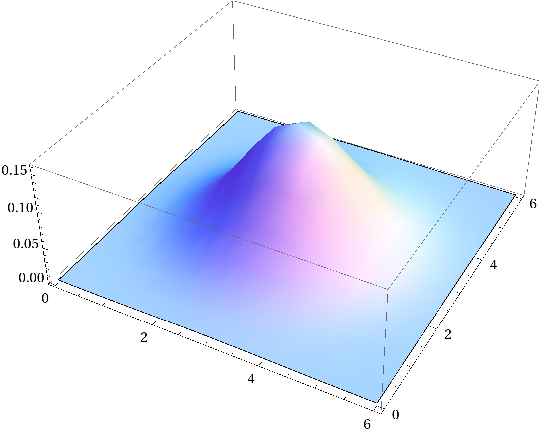
\includegraphics[width=5cm]{2dnormal.pdf}
%$~~$
%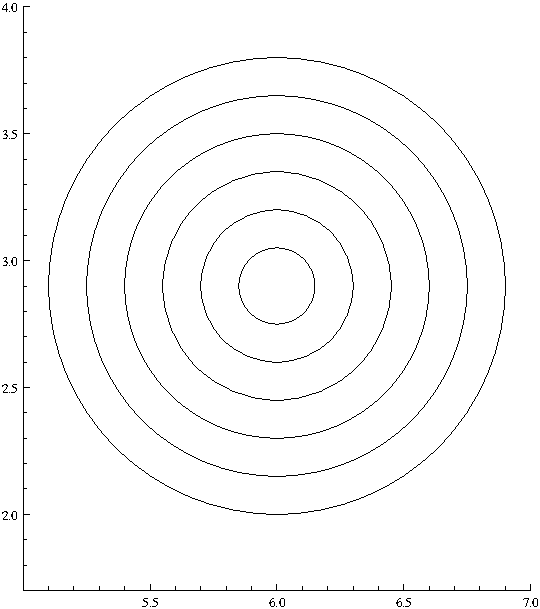
\includegraphics[width=5cm]{2dcontour.pdf}
%\end{figure}

%\end{frame}

%\begin{frame}{Ennen kuin jatketaan 2}

%\begin{itemize}
%\item Useampiulotteisen normaalijakauman karakterisoi kovarianssimatriisi $\boldsymbol{\Sigma}$
%\item $\mathcal{N}_k(\boldsymbol{\mu}_0,\boldsymbol{\Sigma})$, jossa $\boldsymbol{\Sigma} \in \mathbb{R}^{k \times k}$
%\item Neliömatriisi, diagonaalilla varianssit eri dimensioissa
%\item Muut alkiot kertovat dimensioiden välisen kovarianssin
%\end{itemize}

%\end{frame}

\begin{frame}{Data assimilation}

\begin{itemize}
\item Gives an answer to the problem: How to merge measurement and model data in an optimal way?
\item Traditional applications: Weather prediction, oceanography
\item Multiple different methods: 3D- and 4DVar, the family of Kalman filters, ...
\item In this work \emph{Ensemble Kalman Filter}
\end{itemize}

\end{frame}

%\begin{frame}{Data-assimilaatio, yleistä}

%\begin{itemize}
%\item Systeemin (todellinen) tila $\boldsymbol{\psi}^t \in \mathbb{R}^N$
%\item Mittaus $\boldsymbol{d} \in \mathbb{R}^M$
%\begin{itemize}
%\item Ei tarkka
%\item Suhde tilaan $\boldsymbol{d} = \mathbf{M}\boldsymbol{\psi}^t+\boldsymbol{\epsilon}$
%\item Mittamatriisi $\mathbf{M} \in \mathbb{R}^{M \times N}$
%\item Virhe $\boldsymbol{\epsilon} \sim \mathcal{N}_M(0,\boldsymbol{\Sigma})$
%\item Kovarianssimatriisi $\boldsymbol{\Sigma} \in \mathbb{R}^{M \times M}$
%\end{itemize}
%\item Ennustettu tila $\boldsymbol{\psi}^f \in \mathbb{R}^N$
%\begin{itemize}
%\item Aluksi esim. mittauksien perusteella
%\end{itemize}
%\end{itemize}

\begin{frame}{Ensemble Kalman Filter}

\begin{itemize}
\item System is characterized by a bunch of state vectors $\boldsymbol{\psi} \in \mathbb{R}^n$
\item They estimate the same \emph{true} state and their deviation characterizes the uncertainty
\item This group of states is known as \emph{ensemble} 
\item Each member of the ensemble is integrated forwards in time to the next measurement point
\item After the time integration each state is merged with the measurement using
\[
\boldsymbol{\psi}^a = \boldsymbol{\psi}^f + \boldsymbol{\Sigma}_\psi \mathbf{M}^\mathrm{T} \left(\boldsymbol{\Sigma}_d+\mathbf{M}\boldsymbol{\Sigma}_\psi\mathbf{M}^\mathrm{T}\right)^{-1}\left(\boldsymbol{d}-\mathbf{M}\boldsymbol{\psi}^f\right)
\]
\end{itemize}

\end{frame}

\begin{frame}{Ensemble Kalman Filter, estimating parameters}

\begin{itemize}
\item Using the same procedure as previously but extend each state vector with the unknown parameters
\item Formulation of the method guarantees that the unknown parameters are found
\item Note! There must be some kind of correlation between the state and the unknown parameters
\end{itemize}

\end{frame}

\begin{frame}{Back to the problem}

\begin{itemize}
\item Model
\begin{figure}
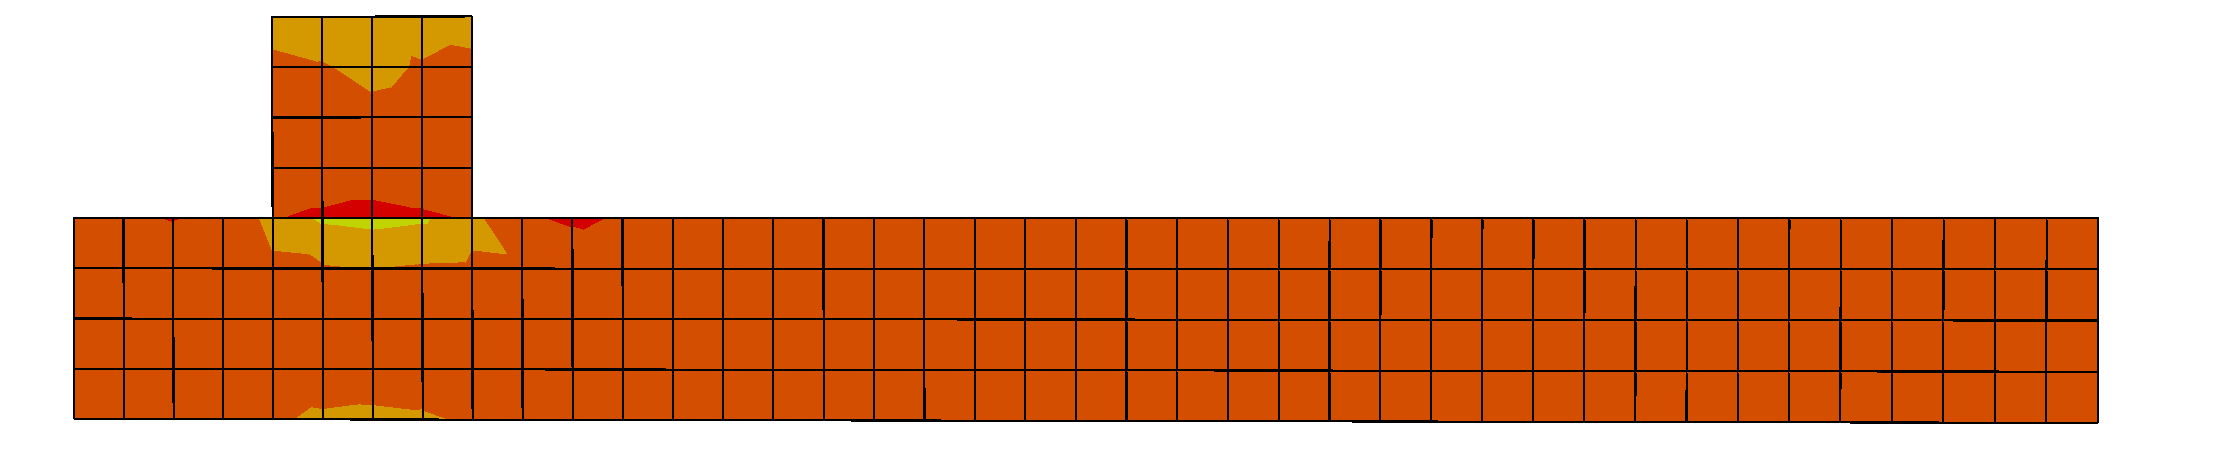
\includegraphics[width=3.3cm]{anim1.pdf}
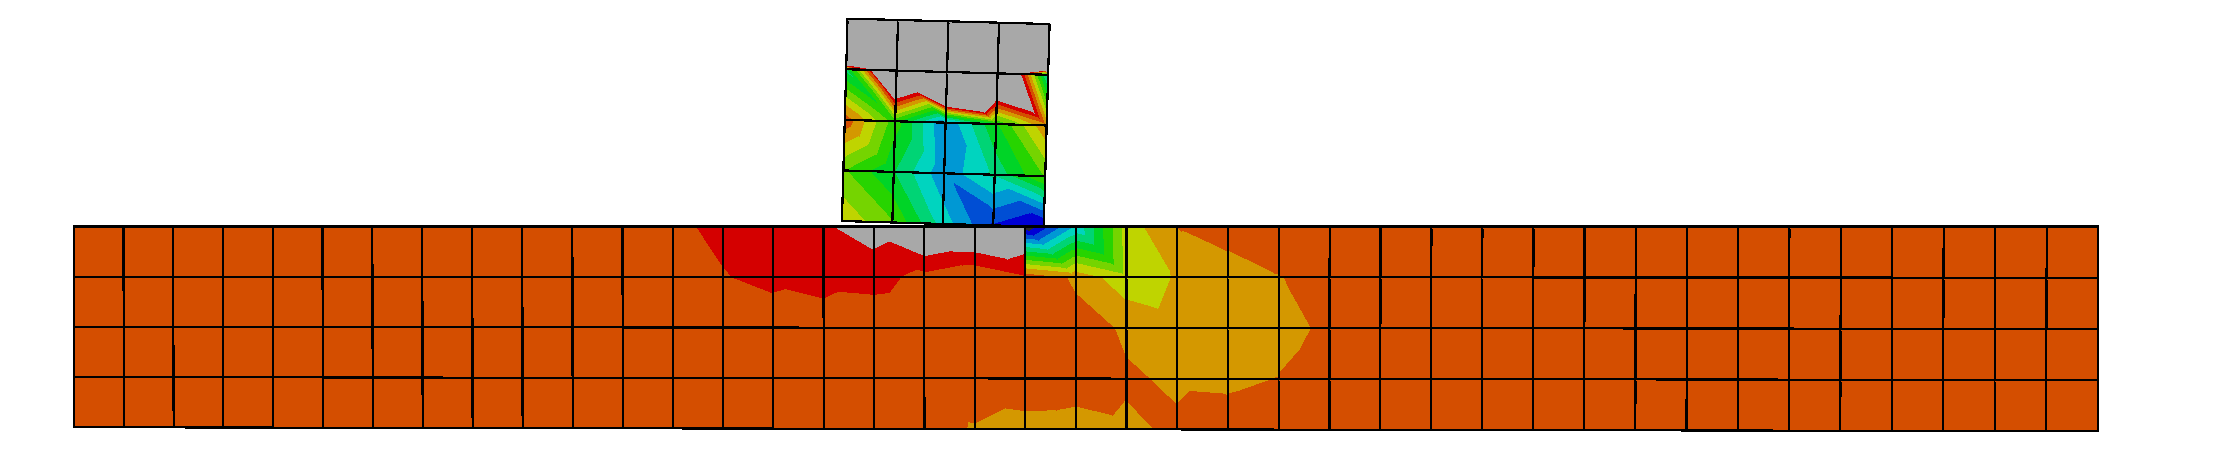
\includegraphics[width=3.3cm]{anim3.pdf}
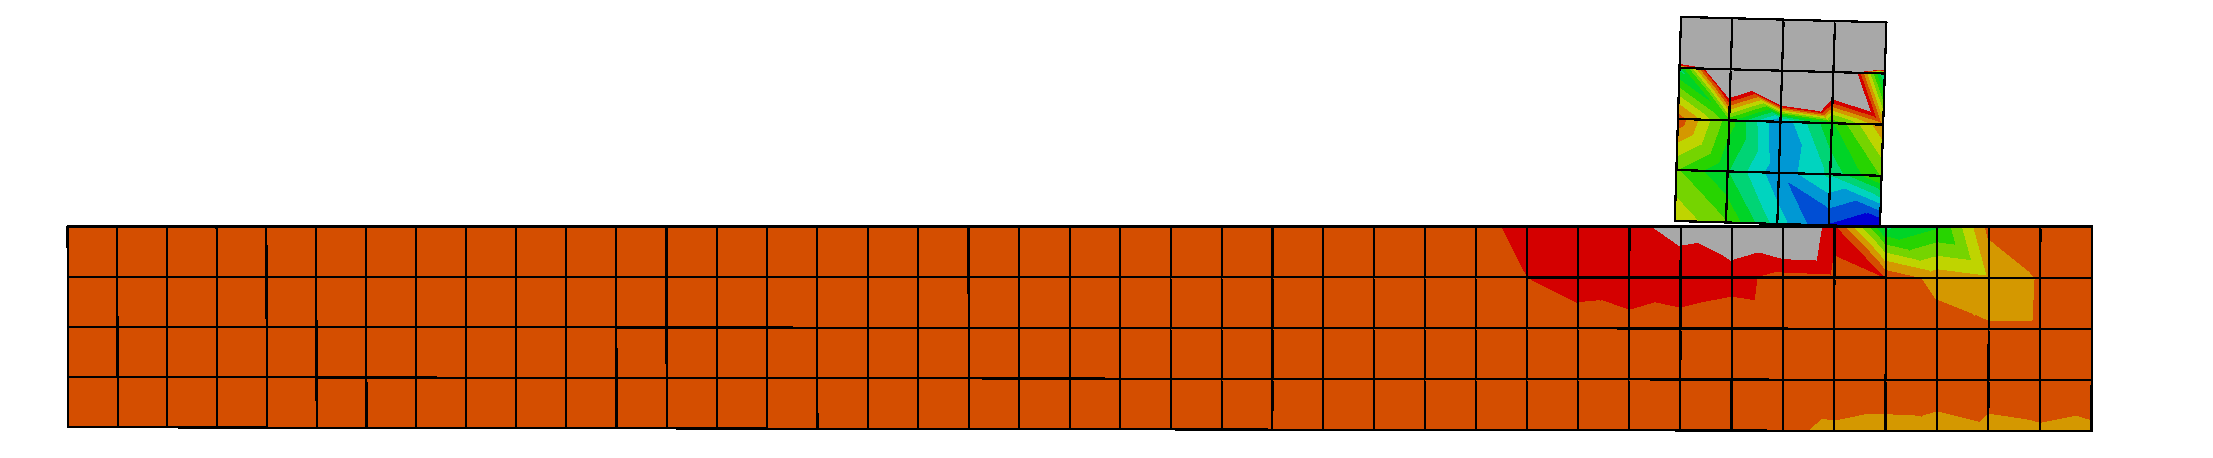
\includegraphics[width=3.3cm]{anim5.pdf}
\end{figure}

\item Estimated parameter $\mu$
\item Define the state as
\[
  \boldsymbol{\psi} = (\sigma_x^1, \sigma_x^2, \sigma_x^3, \dots, \sigma_x^N, \mu)^\mathrm{T}
\]
\item No contact in the beginning $\Rightarrow$ all the stress components are zero
\item Therefore, initial state is specified by $\mu_0$
\end{itemize}

\end{frame}

\begin{frame}{Back to the problem 2}

\begin{itemize}
\item What we need is
\begin{itemize}
\item First-guess $\mu_0=0{,}6$
\item Deviation for first-guess $\sigma_0 = 0{,}1$
\item Ensemble size $n=200$
\item Initial ensemble taken from distribution $\mathcal{N}(\mu_0,\sigma_0^2)$
\end{itemize}
\item A single state of the initial ensemble
\[
\boldsymbol{\psi}_j = (\underbrace{0, 0, \dots, 0, 0,}_{N~\text{kpl}} \mu_0 + \epsilon )^\mathrm{T},~j=1,\dots,n
\]
\item Measurement data when block's displacement is $\Delta x = 7,14,21,\dots,70$ (cm)
\item Measurement data is synthetic
\end{itemize}

%\begin{itemize}
%\item Alussa ei jännityksiä, joten alkutilan määrää ainoastaan $\mu_0 = 0{,}6$
%\item Oletetaan jokin virhe; tässä $\sigma_0 = 0{,}1$ 
%\item Päätetään kokoelman koko, esim. $n=200$
%\item Generoidaan alkukokoelma jakaumasta $\mathcal{N}(\mu_0,\sigma_0^2)$
%\item Alkukokoelman yksittäinen tila muotoa
%\[
%\boldsymbol{\psi}_j = (\underbrace{0, 0, \dots, 0, 0,}_{N~\text{kpl}} \mu_0 + \epsilon )^\mathrm{T},~j=1,\dots,n
%\]
%\item Mitta"hetket": Yläreunan siirtymä $\Delta x = 7,14,21,\dots,70$
%\item Simuloidaan seuraavaan mittahetkeen asti ja yhteensulautetaan mittaus ja kokoelma $\Rightarrow$ kitkakertoimen estimaatti
%\item Mittahetkiä 10, estimaatteja 10
%\end{itemize}

\end{frame}

\begin{frame}{Some results, $n=200$}

\begin{figure}
\begin{tikzpicture}
\node[above right] (img) at (0,0) {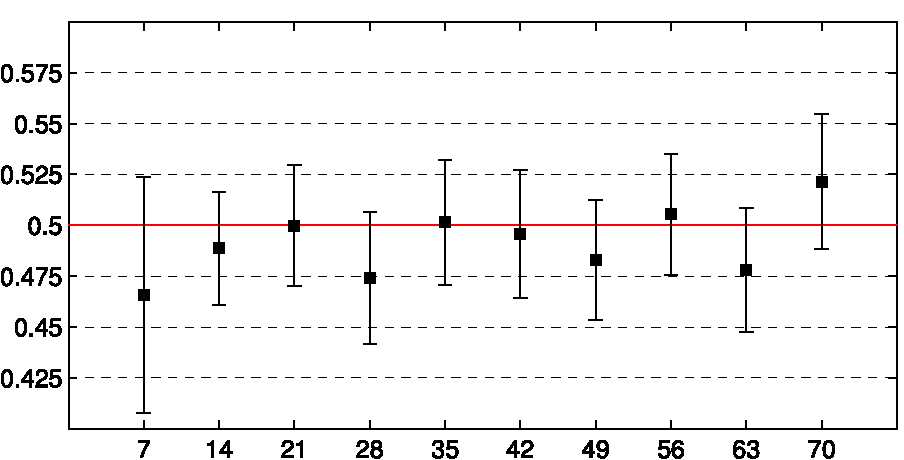
\includegraphics[width=7cm]{xxx_200_no_model_error.pdf}};
\node at (230pt,55pt) {$\mathbf{Q}=\mathbf{0}$};
\end{tikzpicture}
\end{figure}
\vspace{-0.5cm}
\begin{figure}
\begin{tikzpicture}
\node[above right] (img) at (0,0) {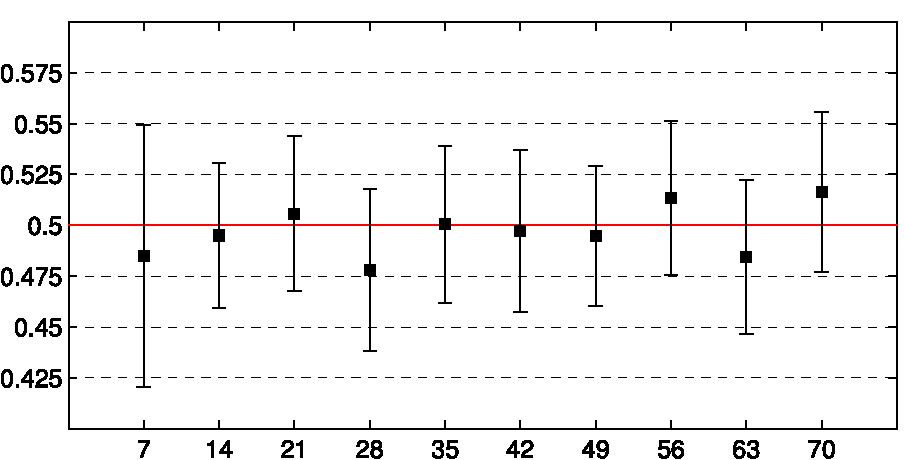
\includegraphics[width=7cm]{xxx_200_model_error.pdf}};
\node at (230pt,55pt) {$\mathbf{Q}=\mathbf{I}\sigma$};
\end{tikzpicture}
\end{figure} 

%\begin{figure}
%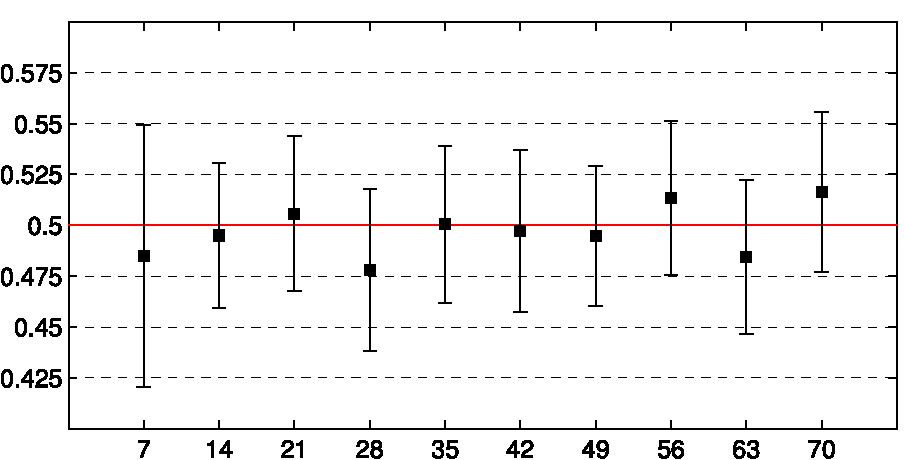
\includegraphics[width=7cm]{xxx_200_model_error.pdf}
%\end{figure}

%\begin{figure}
%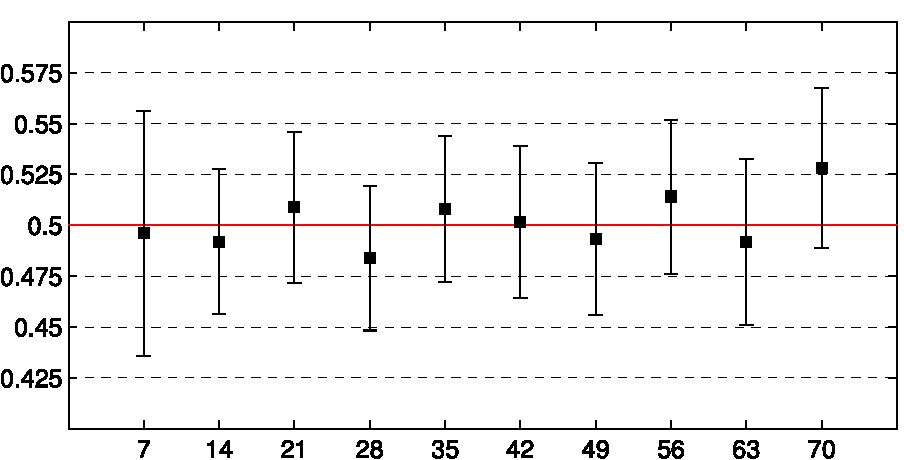
\includegraphics[width=7cm]{xxx_1000_model_error.pdf}
%\end{figure}

\end{frame}

\begin{frame}{Influence of ensemble size, mean}

Red: $\Delta x=70$, blue: $\Delta x=42$, green: $\Delta x=14$

\begin{figure}
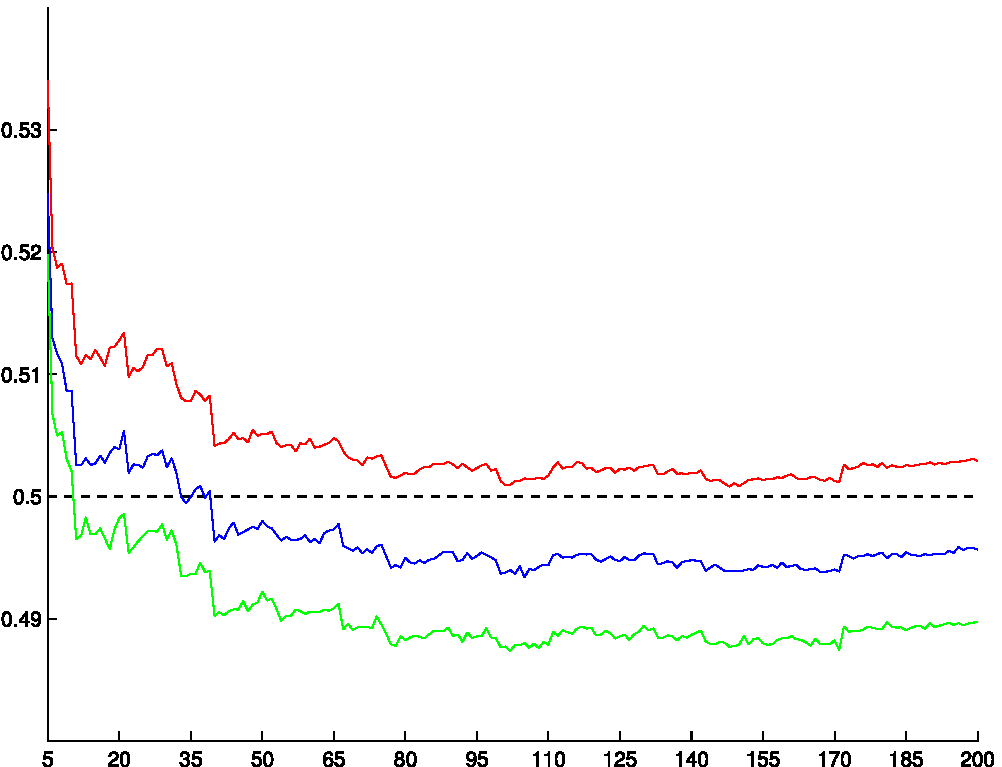
\includegraphics[width=9cm]{mean_conv_2_6_10.pdf}
\end{figure}

\end{frame}

\begin{frame}{Standard deviation of the analysed ensemble}

\begin{figure}
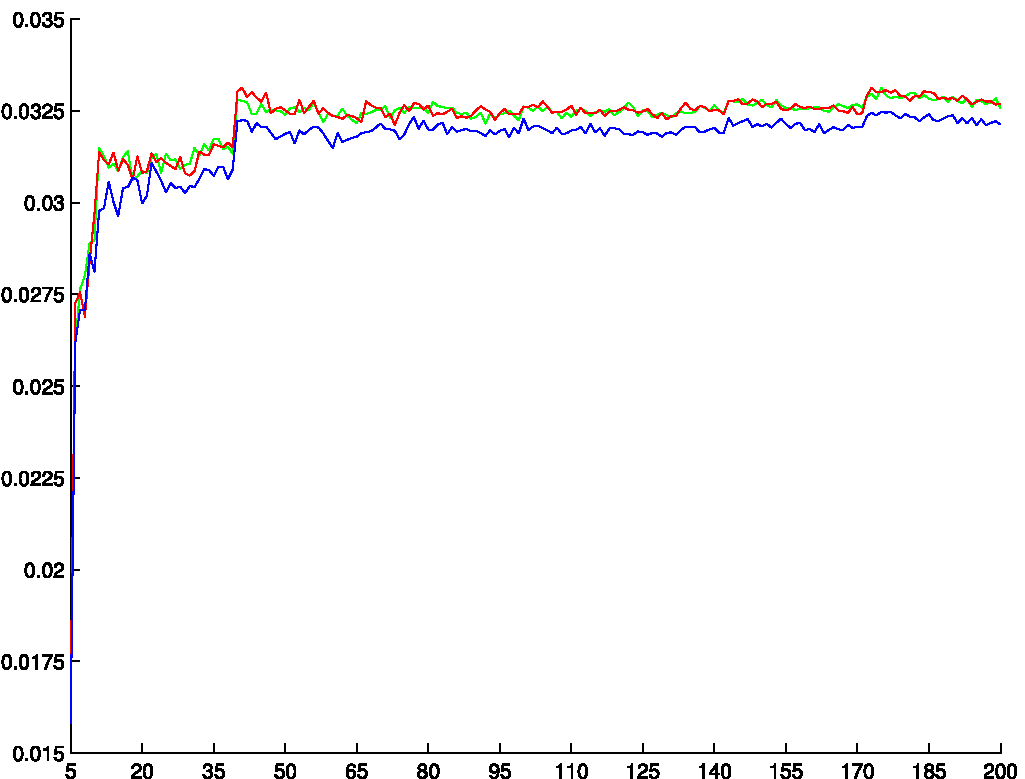
\includegraphics[width=9cm]{ensemble_stdev.pdf}
\end{figure}

\end{frame}

\begin{frame}{Variance between consecutive analyses}

\begin{figure}
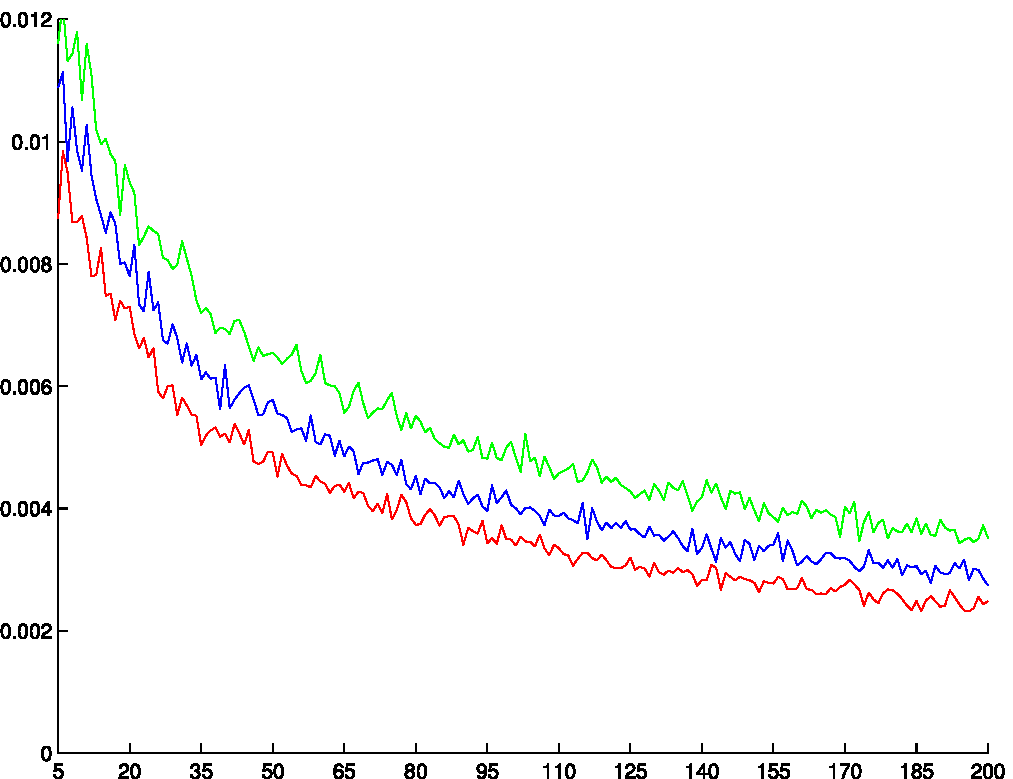
\includegraphics[width=9cm]{stdev_between_analysis.pdf}
\end{figure}

\end{frame}

\begin{frame}{Any questions?}


\end{frame}

\end{document}
